\documentclass[journal,onecolumn]{IEEEtran}
\renewcommand{\baselinestretch}{1.45}
\setlength{\parindent}{0pt}


\usepackage{mathrsfs}
\usepackage{booktabs}
\usepackage{cite}
\usepackage[justification=centering]{caption} % Center the caption
\usepackage{amssymb}
\usepackage{amsmath}
\usepackage{graphics}
\usepackage{color}
\usepackage{epsfig}
\usepackage{graphicx}
\usepackage{amsthm}
\usepackage{float}
\usepackage{subfigure}
\usepackage{amsmath}
\usepackage{amsfonts}
\usepackage{placeins}
\usepackage{lettrine} % Package for dropped capital letters


\allowdisplaybreaks[4]

\title{\LARGE Data-Driven Model Free Adaptive Sliding Mode Control for Multi DC-Motors Speed Regulation}

\author{Tony Blaise Bimenyimana}

\begin{document}
\maketitle

% ---------------------------------------------------------------

\begin{abstract}
    This paper proposes the distributed data-driven sliding mode control approach to address the consensus problem of nonlinear multi-agent systems. Firstly, the equivalent data model for each agent is constructed using the compact-form dynamic linearization (CFDL) technique. Secondly, the novel sliding surface is employed to ensure that the distributed measurement error is bounded through an appropriate stability-guaranteeing mechanism using the input-output data of each agent. Subsequently, to achieve consensus tracking, a distributed model-free adaptive sliding mode controller scheme is developed. Finally, the effectiveness of the proposed control strategy is verified through experiments on multi-DC motors.
\end{abstract}

\section*{Keywords}
Model-free adaptive sliding mode control, compact form dynamic linearization, nonlinear multi-agent system, data-driven control.




\section{Introduction}\label{section:1}

\lettrine{M}otivated by the coordinated behaviors observed in nature, such as bird flocking or herd migration, the distributed control multi-agent systems(MASs) has been studied with interest in recent years.\cite{1} Because of the distributed and flexible structure, the MASs based approaches have significant potential in addressing coordination challenges for complex systems\cite{2}. The control of DC motors is essential in numerious technological applications, with single DC motor serving as the foundation for the systems in various fields, including vehicle coorporation\cite{3}, multi-robot systems and industrial machinery\cite{4}. 

It is challenging to establish an accurate mathematical model for the speed regulation of multi-DC motor systems due to their nonlinear, time-varying, and multi-variable conditions\cite{7}. Even if a relatively accurate mathematical models are developed, the associated control algorithms can become highly complex, so the model-based control approach is difficult to apply or extend to such systems. Nowdays, data-driven methods have been used to control, decision making, planing, fault diagnosis, predicting, etc. In\cite{15}-\cite{16}, a compact form dynamic linarization (CFDL) data-driven modeling method is proposed for nonlinear systems. So far, the CFDL data-driven modeling method has proven to be highly useful in various domains\cite{17}-\cite{20} with different characteristics such as simplicity and particularly, a small amount of calculation, ease of implementation, and strong robustness, making it highly effective for addressing unknown nonlinear time-varying systems.

In\cite{21}, a model-free adaptive control (MFAC) approach is presented for MASs, which uses input and output data to achieve consensus tracking trajectory.

Alternatively, the sliding mode control (SMC) adapts dynamically the system operation based on the current state of the system such as the error and its derivative, ensuring the system follows a predetermined sliding surface\cite{22}. Because the sliding surface can be designed and has the purpose to deal with the object parameters and disturbances, the SMC provides the fast response, insensitivity to parameter changes and disturbances, and simplicity in implementation. The above advantages make SMC widely used in control systems and one of main topic to focus in the ongoing research.\cite{28}-\cite{30}

Inspired by the abovementioned considerations, this paper studies a novel model-free adaptive sliding mode control for speed regulation of multi-DC motors. The proposed control method consists to eliminates the need for precise system models by dynamically adjusting the control law\cite{21}, where is particularly useful in systems where obtaining a detailed model is impractical or complex such as the tradition PID control method. Compared with other existing literature on multi-DC motors systems, the results of this paper have following distinct features.

\begin{enumerate}

    \item The proposed method integrates encoder counts based on the well known constant elapsed time (CET) method\cite{31} for accurate speed control in nonlinear, time-varying multi-DC motor systems. This innovation greatly enhances resolution and reliability, setting it apart from traditional methods.
    
    \item The implementation of a fixed communication topology for agents interconnections, which makes the controller more applicable and flexible in real implementation.
    
    \item Utilizes the pseudo partial derivative (PPD) estimation mechanism within the MFASMC scheme, which provides strong robustness

\end{enumerate}



    The following sections will outline the remaining content of this paper:
    section II provides preliminaries and problem formulation, Section III The main results, Section IV presents simulation results and performance analysis, demonstrating the efficacy of the proposed method under various operating conditions.
    At the end, Section V concludes the paper, summarizing the key findings potential points for future research.
% -----------------------------------------------------------------------------


\section{Preliminaries and problem formulation}\label{section:2}
\subsection{Directed Graph Theory}

The directed graph $ \mathcal{G} = (\mathcal{V}, \mathcal{E}, \mathcal{A}) $ is employed to describe the information exchange between agents. Here, $ \mathcal{A} = [a_{ij}] \in \mathbb{R}^{N \times N} $ represents the adjacency matrix, $ \mathcal{V}=\{v_1, v_2,\dots,v_N\} $ is the set of vertices, and $ \mathcal{E} = [(v_j,v_i)|v_i \in \mathcal{V} ] \subseteq \mathcal{V} \times \mathcal{V}$ is the set of edges. Moreover, $ \mathcal{N}(i) = \{j \in \mathcal{V} |(i,j) \in \mathcal{E}\} $ denotes the neighbor set of agent $ i $, where $ a_{i j} \neq 0$. No self-loop is allowed in this article, which means $(i, i) \notin \mathcal{E}$ for any $ i \in \mathcal{V} $, $ a_{ii}=0$. Furthermore, the degree matrix $ K = diag(k_1,\dots,k_N)$. If $ k_i > 0$, agent $ i $ can directly obtain the information from the leader. The Laplacian matrix $ L $ is defined as $ L = (\mathcal{D}-\mathcal{A})$, here $\mathcal{D} = diag({d_1,\dots,d_N})$ and $d_i=\sum_{j=1}^{N} a_{i j}$ denotes the in-degree matrix. Moreover, the graph is strongly connected if the path exists between every pair of vertices.

\subsection{Problem Formulation}

Consider the nonlinear multi-agent systems composed of $ N $ agents:

\begin{equation}
    \label{model 1}
    y_i(k+1) = f_i(y_i(k), u_i(k)), \quad i = 1, 2, \dots, N
\end{equation}

% \noindent 
where $u_i(k) \in \mathbb{R}$ and $y_i(k) \in \mathbb{R}$ represent the system input and output signals of agent $ i $, respectively. $f_i(\cdot)$ signifies an unknown nonlinear function.

Assumption 1: The partial derivative of \( f_i(\cdot) \) with respect to \( u_i(k) \) is continuous.

Assumption 2: The system (\ref{model 1}) satisfies the generalized Lipschitz condition, meaning that if \( \Delta u_i(k) = u_i(k) - u_i(k - 1) \neq 0 \) then \( | \Delta y_i(k + 1) | \leq b |\Delta u_i(k)| \) holds for any \( k \), where \( \Delta y_i(k + 1) = y_i(k + 1) - y_i(k) \).
 

% Under Assumptions 1 and 2, the unknown agent dynamics (\ref{model 1}) can be transformed into the following dynamic linearization model and then the distributed control law will be designed based on it:

Remark 1: The assumptions above are general. As the common condition for model-free control methods, Assumption 1 is crucial in ensuring effective system performance. Assumption 2 implies that the system input rate constrains the system output rate, which is satisfied in many practical systems.

Lemma 1\cite{8}: Consider the nonlinear multi-agent system (\ref{model 1}) satisfying above two assumptions. If $ | \Delta u_i(k) | \neq 0 $ holds, then the system can be transformed into the CFDL data model as follows:


\begin{equation}
    \label{model 2}
    \Delta y_i(k+1)=\phi_i(k)\Delta u_i(k)
\end{equation}

where \(\phi_i(k)\) is called pseudo partial derivative (PPD), satisfying \( | \phi_i(k) | \leq b\).

Remark 2: The CFDL technique does not contain any prior knowledge about the system dynamic model. Moreover, the dynamic behavior of time-varying PPD can be highly complex and more challenging to verify. Therefore a data-driven approach to study numerical characteristics becomes the preferred solution.
 
The distributed measurement error of \(\xi_i(k)\) for $N$ agents is established as:

\begin{equation}
    \label{model 3}
    \xi_i(k) = \sum_{j \in N_i} a_{ij}( y_j(k)-y_i(k)) + d_i(y_d(k) - y_i(k ))
\end{equation}

if the agent $ i $ can receive data from the leader, then $d_i=1$; otherwise, $d_i=0$. Additionally, $y_d(k)$ represents the reference trajectory. 

 

\section{Main Results}

\subsection{Model Free Adaptive Controller Design}


\begin{figure}[H]
    \centering
    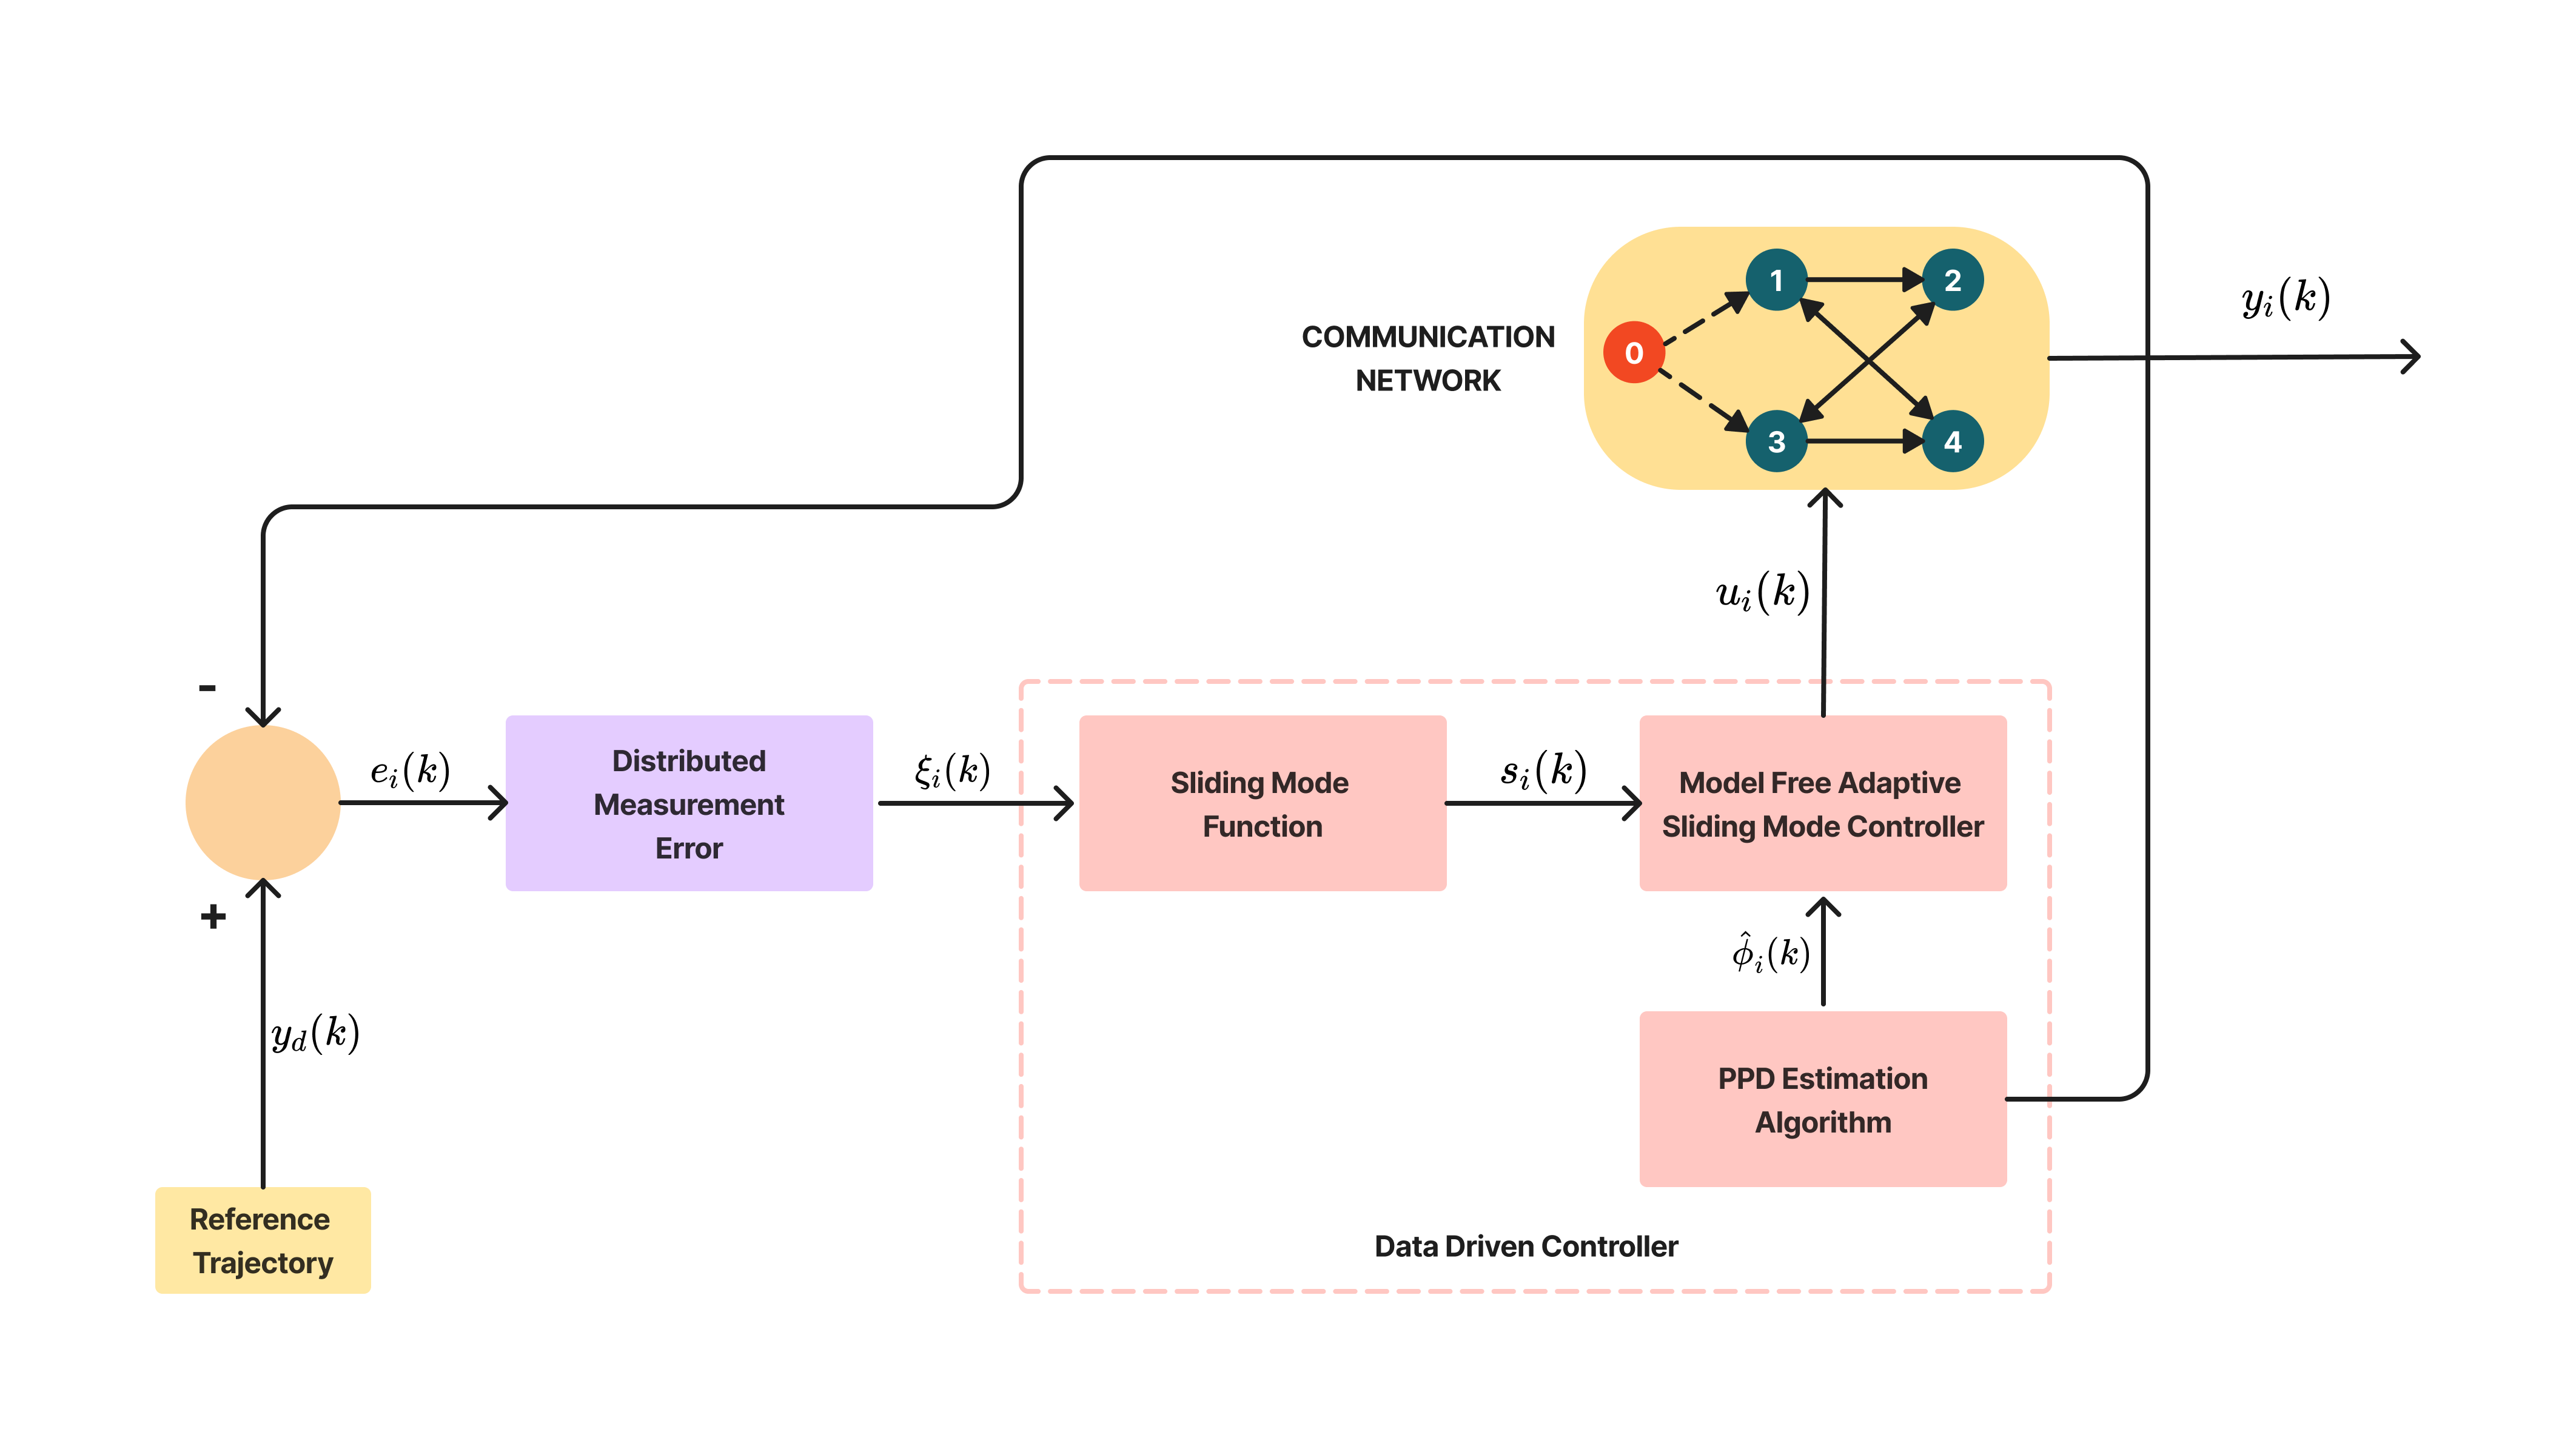
\includegraphics[width=0.9\textwidth]{diagram.png}
    \caption{Block diagram.}
    \label{fig:diagram} % Label for referencing the figure
\end{figure}


Consider the following PPD criterion function, which is used to evaluate the performance of the parameter \(\phi_i(k)\):

\begin{equation}
    \label{model 4}
    J(\phi_i(k)) = | \Delta y_i(k) - \phi_i(k)  \Delta u_i(k-1)|^2 + \mu |\phi_i(k) - \hat{\phi}_i(k-1)|\
\end{equation}

Assumption 4 : The PPD \(\phi_i(k) > \varsigma\) , \(i = 1,2,3, \dots, N\) holds for all \(k\), where \( \varsigma \) is an rondomly small positive constant without loss of generality, assume that \(\phi_i(k) > \varsigma\).


Differentiating equation (\ref{model 4}) with respect to PPD parameter \(\phi_i(k)\) and make it equal to zero, the following update rule is proposed for the distributed MFAC algorithm:


% \begin{equation}
%     \label{model 5}
%     \frac{\partial J({\phi}_i(k))}{\partial {\phi}_i(k)} = | \Delta y_i(k) - \hat{\phi}_i(k)  \Delta u_i(k-1)|^2 + \mu |\hat{\phi}_i(k) - \hat{\phi}_i(k-1)| = 0
% \end{equation}


% And, let's compute the derivative of \( J(\hat{\phi}_i(k)) \), we obtain:

% \begin{equation}
%     \label{model 6}
%     2 [ \Delta y_i(k) - \phi_i(k-1)] - [\Delta u_i(k-1)] + 2 \mu [\phi_i(k) -  \hat{\phi}_i(k-1)] = 0
% \end{equation}

% This equation provides a necessary condition for minimizing the criterion function \(J(\phi_i(k))\) and based on this optimization criterion,



\begin{equation}
    \label{model eq:ppd_parameter}
    \hat{\phi}_i(k) = \hat{\phi}_i(k-1) + \frac{\eta \Delta u_i(k-1) (\Delta y_i(k) - \hat{\phi}_i(k-1) \Delta u_i(k-1))}{\mu + \Delta u_i(k-1)}
\end{equation}

\begin{equation}
    \label{reset}
    \hat{\phi}_i(k) = \hat{\phi}_i(1),  \text{    if}  |\hat{\phi}_i(k) | \leq \epsilon \ or \ sign(\hat{\phi}_i(k)) \neq  sign(\hat{\phi}_i(1))
\end{equation}

Here, $\eta$ is the learning rate that controls the step size of the update, $\mu > 0$ is a weight factor. $ \hat{\phi}_i(1) $ is the initial value of $ \hat{\phi}_i(k)$ and $ \hat{\phi}_i(k)$ is the estimated value of $ \phi_i(k)$.

Remark 3: In the parameter estimation law (\ref{model eq:ppd_parameter}), $y_i(k) $ is used to estimate $\hat{\phi}_i(k)$. The abovementioned scheme ensures the convergence of (\ref{model eq:ppd_parameter}). Additionally, the reset algorithm (\ref{reset}) is introduced to enhance the ability of the parameter estimation algorithm to effectively track time-varying parameters.


To design the MFAC alogrithm, the performance function \(J(u_i(k))\) is set as:

\begin{equation}
    \label{model 9}
    J(u_i(k)) = |\xi_i(k+1)|^2 + \lambda|u_i(k) - u_i(k-1)|^2
\end{equation}

Subtituting (\ref{model 2}) and (\ref{model 3}) into (\ref{model 9}), then differentiating (\ref{model 9}) with respect to \(u_i(k)\), and make it equal to zero, gives:

\begin{equation}
    \label{model eq:mfac}
    u_{i,\text{MFAC}}(k) = u_{i,\text{MFAC}}(k - 1) + \frac{\rho \phi_i(k)}{\lambda + |\phi_i(k)|^2} \xi_i(k)
\end{equation}


where \(\rho\) \(\in\) (0,1) is a step-size constant, which is added to make (\ref{model eq:mfac}) general. Using the parameter estimation algorithm (\ref{model eq:ppd_parameter}) and the control law algorithm (\ref{model eq:mfac}), the MFAC scheme is constructed. 


\subsection{Sliding Mode Controller Design}






% y_i(k + 1) = f_i(y_i(k), u_i(k)), \quad i = 1, 2, \ldots, N

To design the SMC for system, the sliding mode surface is first defined, guiding the behavior of system to ensure robust and accurate tracking of the desired trajectory.

The sliding mode surface is defined as:

\begin{equation}
    \label{model eq:sms}
    S_i(k+1) = S_i(k)+e_i(k+1)+\alpha e_i(k) 
\end{equation}

where \(\alpha\) is a positive constant, and  to ensure that the system trajectory is driven toward and remains on the sliding surface. The reaching law dictates how quickly the system state converges to the sliding surface and is given by:

\begin{equation}
    \label{model eq:reaching_law}
    \Delta S_i(k+1) = - \varepsilon T sign(k) 
\end{equation}

In that equation, \(\varepsilon\) is a small positive constant that controls the rate of the convergence, \(T\) is the sampling period, and \(sign(k)\) indicates the direction in which the system should move to reach the sliding surface.

By combining the sliding surface definition and the reaching law, derivating the control law that ensures the desired tracking performance while maintaining robustness.

The final sliding mode control input \(u_{i,\text{SMC}}(k)\) is designed:

\begin{equation}
    \label{model eq:smc}
    u_{i,\text{SMC}}(k) = u_{i,\text{SMC}}(k) + \frac{y_d(k+1)-y(k) + \alpha e_i(k) + \varepsilon T sign(k)}{\phi_i(k)}
\end{equation}

To enhance the  adaptibility of the control system, the MFASMC approach is employed.  the conrol input of the system is defined as:

\begin{equation}
    \label{model eq:mfasmc}
    u_i(k) = u_{i,\text{MFAC}}(k) + \Gamma_i  u_{i,\text{SMC}}(k)
\end{equation}

where the parameter \(\Gamma\) is a gain factor that adjusts the contribution of the sliding mode control in the control effort and tunes the convergence rate.

\subsection{Stability Analysis}

The stability analysis is conducted in two primary steps. The first step focuses on estabilishing the bounds, the second step ensures that the error remains within acceptable limits over time, leading to a stable system.

Step 1: Establishment of error bounds

The estimated error between the estimated and actual values of the system parameters, denote as \(\tilde{\phi_i}(k)
=\hat{\phi}_i(k)-\phi_i(k) \), starting from the foundational equation derived from the compact dynamic linearization model in equation (\ref{model 2}) along with the PPD estimation equation (\ref{model eq:ppd_parameter}). To ensure the theorem validity, the detailed proof that demonstrates the correctness of this error bound is provided.

\begin{equation}
    \label{model 15}
    \tilde{\phi_i}(k) = \hat{\phi_i}(k+1) + \frac{\eta \Delta u_i(k-1)}{\mu + | \Delta u_i(k-1)|^2}  ((\Delta y_i(k) - \hat{\phi_i}(k-1)\Delta u_i(k-1) )) - \phi_i(k)
\end{equation}

Then by simplifying the previous equation, the result is:


% \begin{equation}
%     \label{model 19}
%     \beta_i(k) =  \frac{\eta \Delta u_i(k-1)}{\mu + | \Delta u_i(k-1)|^2}
% \end{equation}

The control coefficient \(\beta_i(k)\) is expressed from the previous equation, plays a critical role in adjusting the control input for each agent at time step $k$. The following equation is expressed:

 
\begin{equation}
    \label{model 17}
    \tilde{\phi_i}(k) = \tilde{\phi_i}(k-1)+\beta_i(k)  (\Delta y_i(k) - \hat{\phi_i}(k-1)\Delta u_i(k-1) -\phi_i(k) - \phi_i(k-1))
\end{equation}

% \begin{equation}
%     \label{model 18}
%     \tilde{\phi_i}(k) = (1-\frac{\eta(\Delta u_i(k-1))^2}{\mu + |\Delta u_i(k-1)|^2})\tilde{\phi_i}(k-1) + \phi_i(k-1) - \phi_i(k)
% \end{equation}

\begin{equation}
    \label{model 19}
    \tilde{\phi_i}(k) = (1-\frac{\eta(\Delta u_i(k-1))^2}{\mu + |\Delta u_i(k-1)|^2})\tilde{\phi_i}(k-1) - \Delta \phi_i(k)
\end{equation}

% To prove the boundedness of the error, we begin by taking the absolute value of each term in the error equation (\ref{model 22}). This step is crucial as it allows us to establish an inequality that provides an upper bound on the error.

% Taking the absolute value on both sides and applying the triangle inequality to the right-hand side, we obtain:

% \begin{equation}
%     \label{model 23}
%     |\tilde{\phi_i}(k)| \leq  |(1-\frac{\eta(\Delta u_i(k-1))^2}{\mu + |\Delta u_i(k-1)|^2})|*|\tilde{\phi_i}(k-1) |- |\Delta \phi_i(k)|
% \end{equation}

% Let,
% \begin{equation}
%     \label{model 24}
%     \alpha(k-1) = \frac{\eta(\Delta u_i(k-1))^2}{\mu + |\Delta u_i(k-1)|^2}
% \end{equation}

% So:

% \begin{equation}
%     \label{model 25}
%     |\tilde{\phi_i}(k)| \leq  |(1-\alpha(k-1))|*|\tilde{\phi_i}(k-1) |- |\Delta \phi_i(k)|
% \end{equation}

% Since \(\Delta u_i(k) \neq  0\), \(0 < \eta \leq 1 \) and \(\mu \geq 0 \), \(0 < \alpha(k-1) \leq q_1 < 1  \)

% Upper bound for \(1-\alpha(k-1) \) by replacing it with constant \(q_1\), we get:

% \begin{align}
%     \label{model 26}
%     |1-\alpha(k-1)| &\leq 1-q_1 \\
%     |\Delta \phi_i(k)| \leq |\phi_i(k-1) - \phi_i(k)| \leq b 
% \end{align}

% By combining the inequalities and applying an iterative process, we obtain the following expression:

% \begin{equation}
%     \label{model 28}
%     |\tilde{\phi_i}(k) \leq |1-q_1||\tilde{\phi_i}(k-1)|+b
% \end{equation}
% \begin{equation}
%     \label{model 29}
%     |\tilde{\phi_i}(k-1) \leq |1-q_1||\tilde{\phi_i}(k-2)|+b
% \end{equation}

% continuing the process back to the initial condition(0) , with sum of geometric series of \(\sum_{j=o}^{k-1} (1-q_1)^j = \frac{1-(1-q_1)^k}{q_1} \)

% Thus:
% \begin{equation}
%     \label{model 30}
%     |\tilde{\phi_i}(k) \leq (1-q_1)^k ((\tilde{phi_i}(0))) + \frac{b}{q_1} (1-(1-q_1)^k)
% \end{equation}

% Simplifying the bound, as \(k=\infty\), so\((1-q_1)^k=0\), therefore \(\tilde{\phi_i}(k) \) is bounded, because if satifies: \(|\tilde{\phi_i}(k) \leq \frac{b}{q_1} \)

To demonstrate the boundedness of the error, by taking the absolute value of both sides of the error (\ref{model 19}). This is a crucial step, as it allows us to establish an inequality that provides an upper bound on the error term.

Taking the absolute value on both sides and applying the triangle inequality to the right-hand side, it follows that:

\begin{equation}
\label{model 20}
|\tilde{\phi_i}(k)| \leq \left| 1 - \frac{\eta (\Delta u_i(k-1))^2}{\mu + |\Delta u_i(k-1)|^2} \right| |\tilde{\phi_i}(k-1)| + |\Delta \phi_i(k)|
\end{equation}

Defining:

\begin{equation}
\label{model 21}
\alpha(k-1) = \frac{\eta (\Delta u_i(k-1))^2}{\mu + |\Delta u_i(k-1)|^2}
\end{equation}

So  (\ref{model 20}) becomes:

\begin{equation}
\label{model 22}
|\tilde{\phi_i}(k)| \leq |1 - \alpha(k-1)| |\tilde{\phi_i}(k-1)| + |\Delta \phi_i(k)|
\end{equation}

% Given that \(\Delta u_i(k) \neq 0\), \(0 < \eta \leq 1\), and \(\mu \geq 0\), it follows that \(0 < \alpha(k-1) \leq q_1 < 1\).

Since $|\phi_i(k)| \leq b $, considering assumption 4, we can obtain $|\phi_i(k-1)-\phi_i(k)|$, and then:

\begin{equation}
\label{model 23}
|\tilde{\phi_i}(k)| \leq |1 - q_1| |\tilde{\phi_i}(k-1)| + b
\end{equation}

% Continuing this process for previous time steps::

% \begin{equation}
% \label{model 24}
% |\tilde{\phi_i}(k-1)| \leq |1 - q_1| |\tilde{\phi_i}(k-2)| + b
% \end{equation}

Back to the initial condition at \(k=0\) and summing the resulting geometric series:
\[
\sum_{j=0}^{k-1} (1-q_1)^j = \frac{1-(1-q_1)^k}{q_1}
\]

Thus:

\begin{equation}
\label{model 25}
|\tilde{\phi_i}(k)| \leq (1 - q_1)^k |\tilde{\phi_i}(0)| + \frac{b}{q_1} (1 - (1 - q_1)^k)
\end{equation}

As \(k \rightarrow \infty\), the term \((1-q_1)^k\) tends to zero, simplifying the bound to:

\begin{equation}
\label{model 26}
|\tilde{\phi_i}(k)| \leq \frac{b}{q_1}
\end{equation}

% Therefore, \(\tilde{\phi_i}(k)\) is bounded by \(\frac{b}{q_1}\), proving that the error remains within this bound as \(k\) approaches infinity.


Remark 4: The inequality in \eqref{model 26} shows that \(\tilde{\phi_i}(k)\) is bounded by \(\frac{b}{q_1}\). This result implies that the error \(\tilde{\phi_i}(k)\) will remain within this bound, even as \(k\) approaches infinity. Thus, the system error behavior is effectively controlled and constrained.

    

% Part 2: The convergence of tracking error , from (\ref{model 3}). \(\xi_i(k)\) can be rewritten in terms of tracking errors as follows:

% \begin{equation}
%     \label{model 32}
%     \xi_i(k) = \sum_{j\epsilon N_i} (e_i(k) - e_j(k))+d_i e_i (k)
% \end{equation}

% \(y(k) =  \begin{pmatrix} y_1 \\ y_2 \\ y_3 \\ \vdots \\ y_n \end{pmatrix} , e(k) =  \begin{pmatrix} e_1 \\ e_2 \\ e_3 \\ \vdots \\ e_n \end{pmatrix}, \xi(k) =  \begin{pmatrix} \xi_1 \\ \xi_2 \\ \xi_3 \\ \vdots \\  \xi_n \end{pmatrix}, u(k) =  \begin{pmatrix} u_1 \\ u_2 \\ u_3 \\ \vdots \\ u_n \end{pmatrix}
% \)

% \begin{equation}
%     \label{model 33}
%     \xi_i(k) = (L+D)e(k) 
% \end{equation}

% with \(D = diag(d_1,d_2,d_3,\dots,d_n)\)

% Where \(u(k) = u(k-1) + \rho*diag(\frac{\hat{\phi_1}(k)}{\lambda + |\hat{\phi_1}(k)|^2},\frac{\hat{\phi_2}(k)}{\lambda + |\hat{\phi_2}(k)|^2},\frac{\hat{\phi_3}(k)}{\lambda + |\hat{\phi_3}(k)|^2},\dots, \frac{\hat{\phi_n}(k)}{\lambda + |\hat{\phi_n}(k)|^2}) (L+D)e(k)\)

% \begin{equation}
%     \label{model 34}
%     u(k) = u(k-1)+\rho H_1(k)(L+D)e(k)  
% \end{equation}

% We can describe (\ref{model 2}) as \(y(k+1) = y(k) + \phi(k) \Delta u(k) \)

% So:

% \(y(k+1) = y(k) + diag(\phi_1(k) \phi_2(k) \phi_3(k) \dots \phi_n(k)) \Delta u(k)\)

% \begin{equation}
%     \label{model 35}
%     y(k+1) = y(k) + H_\phi(k) \Delta u(k)
% \end{equation}

% Where \(\Delta u(k) = u(k)-u(k-1) , H_\phi(k) = diag(\phi_1(k) \phi_2(k) \phi_2(k) \dots \phi_n(k) ) \)

% By Subtituting (\ref{model 34}) into (\ref{model 35}) we can get: \\
% \(e(k+1)-e(k) = y(k) - y(k+1) \) 

% \(e(k+1) = e(k) + y(k) - y(k+1) \\
% e(k+1) = e(k) - H_\phi(k) \rho H_1(k) (L+D) e(k)  
% \)

% Which give as the following equation:

% \begin{equation}
%     \label{model 36}
%     e(k+1) = (I-\rho \sum(k) (L+D))e(k)
% \end{equation}

% Where \(\sum(k) = H_\phi(k) H_1(k) = diag(\frac{\hat{\phi_1}(k)}{\lambda + |\hat{\phi_1}(k)|^2},\frac{\hat{\phi_2}(k)}{\lambda + |\hat{\phi_2}(k)|^2},\frac{\hat{\phi_3}(k)}{\lambda + |\hat{\phi_3}(k)|^2},\dots, \frac{\hat{\phi_n}(k)}{\lambda + |\hat{\phi_n}(k)|^2})
% \\
% =diag(\mathcal{V}_1(k) \mathcal{V}_2(k) \mathcal{V}_3(k) \dots \mathcal{V}_n(k) )
% \)

% With 

% \(\mathcal{V}_i(k) =\frac{\hat{\phi_i}(k)}{\lambda + |\hat{\phi_i}(k)|^2} , i=1,2,3,\dots,n\) 

% Let \(\Theta(k) = \sum(k) (L+D) \) , we get \(e(k+1) = (I-\rho \Theta(k))e(k) \)

% Finnaly , we have:

% \begin{equation}
%     \label{model 37}
%     ||I-\rho \ \Theta(k)|| < 1
% \end{equation}

% so :

% \(\lim{k \rightarrow \infty} ||e(k+1)|| = 0\)

% \section*{Part 2: Convergence of Tracking Error}



%  In this part, delving into the convergence properties of the distributed error \(\xi_i(k)\). To understand the convergence, we start with the expression for \(\xi_i(k)\) as given in equation (\ref{model 3}). Aiming to express \(\xi_i(k)\) in terms of the individual tracking errors \(e_i(k)\) and the errors associated with neighboring systems.
Step 2:

The expression for \(\xi_i(k)\) is formulated as follows:

\begin{equation}
    \label{model 27}
    \xi_i(k) = \sum_{j \in N_i} (e_i(k) - e_j(k)) + d_i e_i(k)
\end{equation}

In this equation, \(\xi_i(k)\) represents the distributed measurement of the $i$th system at time \(k\), taking into account the deviations from the neighbors \(j\) in the set \(N_i\) and an additional term \(d_i e_i(k)\) that depends on the specific characteristics of the $i$th system.

Define the collective stack vectors as follows:

    
\begin{align*}
    y(k)   &= \left[ y_1(k) \quad y_2(k) \quad \dots \quad y_n(k) \right]^T \\
    e(k)   &= \left[ e_1(k) \quad e_2(k) \quad \dots \quad e_n(k) \right]^T \\ 
    \xi(k) &= \left[ \xi_1(k) \quad \xi_2(k) \quad \dots \quad \xi_n(k) \right]^T \\
    u(k)   &= \left[ u_1(k) \quad u_2(k) \quad \dots \quad u_n(k) \right]^T
    \end{align*}
    

Using the above-mentioned definitions, the measurement output \(\xi_i(k)\) can be rewritten as as follows:

\begin{equation}
    \label{model 28}
    \xi(k) = (L + D) e(k)
\end{equation}

Where \(L\) represents the interaction matrix that describes how each system interacts with its neighbors, while \(D\) is a diagonal matrix defined by \(D = \text{diag}(d_1, d_2, d_3, \dots, d_n)\). By noting the definition in (\ref{model 28}), the controller (\ref{model eq:mfac}) is rewritten as:


\begin{equation}
    \label{model 29}
    u(k) = u(k-1) + \rho H_1(k) (L + D) e(k)
\end{equation}

where


\[
H_1(k) = \rho   \text{diag}\left(\frac{\hat{\phi}_1(k)}{\lambda + |\hat{\phi}_1(k)|^2}, \frac{\hat{\phi}_2(k)}{\lambda + |\hat{\phi}_2(k)|^2}, \dots, \frac{\hat{\phi}_n(k)}{\lambda + |\hat{\phi}_n(k)|^2}\right).
\]


% where \(H_1(k)\) is a diagonal matrix whose elements are functions of the estimated parameters \(\hat{\phi}_i(k)\), and \(H_\phi(k)\) is defined as:


In similar way, CFDL model (\ref{model 2}) is also transformed into the following collective form:

\begin{equation}
    \label{new cfdl}
    % e(k+1) = (I - \rho \Theta(k)) e(k)
    y(k+1) = y(k) + H_\phi(k) \Delta u(k)
\end{equation}

where

\[\Delta u(k) = u(k)-u(k-1)\]
\[
H_\phi(k) = \text{diag}(\phi_1(k), \phi_2(k), \phi_3(k), \dots, \phi_n(k))
\]


We can substitute (\ref{model 29}) and (\ref{new cfdl}) to get

\begin{equation}
    \label{model 30}
    % e(k+1) = (I - \rho \Theta(k)) e(k)
    e(k+1) = (I - \rho \sum(k) (L+D)) e(k)
\end{equation}

where $\sum(k) = H_\phi(k)H_1(k) = \text{diag}(\mathcal{V}_1(k), \mathcal{V}_2(k), \mathcal{V}_3(k), \dots, \mathcal{V}_n(k))$, and each \(\mathcal{V}_i(k)\) is given by:

% where \(\Theta(k)\) is defined by:

% \[
% \Theta(k) = \sum(k) (L + D) = H_\phi(k) H_1(k) (L + D)
% \]

% with:

% \[
% \sum(k) = \text{diag}\left(\frac{\hat{\phi_1}(k)}{\lambda + |\hat{\phi_1}(k)|^2}, \frac{\hat{\phi_2}(k)}{\lambda + |\hat{\phi_2}(k)|^2}, \frac{\hat{\phi_3}(k)}{\lambda + |\hat{\phi_3}(k)|^2}, \dots, \frac{\hat{\phi_n}(k)}{\lambda + |\hat{\phi_n}(k)|^2}\right)
% \]

% which can be expressed in diagonal form as:

% \[
% \sum(k) = \text{diag}(\mathcal{V}_1(k), \mathcal{V}_2(k), \mathcal{V}_3(k), \dots, \mathcal{V}_n(k))
% \]



\[
\mathcal{V}_i(k) = \frac{\hat{\phi_i}(k)}{\lambda + |\hat{\phi_i}(k)|^2}, \quad i = 1, 2, \dots, n
\]

Thus :

\[
\Theta(k) = \text{diag}(\mathcal{V}_1(k), \mathcal{V}_2(k), \mathcal{V}_3(k), \dots, \mathcal{V}_n(k)) (L + D)
\]

To ensure convergence of the tracking error, the following condition is imposed:

\begin{equation}
    \label{model 31}
    \|I - \rho \Theta(k)\| < 1
\end{equation}

This condition guarantees that the tracking error \(e(k)\) will approach zero as \(k \to \infty\). Consequently:

\[
\lim_{k \to \infty} \|e(k+1)\| = 0
\]

% This result indicates that the tracking error will converge to zero, demonstrating the effectiveness of the proposed control strategy in achieving desired tracking performance.

Remark 5: This condition ensures that the tracking error decreases over time and eventually converges to zero as $k$ approaches infinity. The implication is under the proposed control strategy, the system will successfully align with the desireed performance, eliminating any discrepancies in tracking. This convergence demonstrates the robutness and effectiveness of the control method in achieving accurate and stable performance.






% \section{Extension to Switching Topology}

% In this section, the proposed design is extendend to the multiagent system with switching topology.

% Let \(\mathcal{G}\) denote a time-varying graph depend on \(k\). The adjacency matrix associated with \(\mathcal{G}(k)\) is denoted by \(\mathcal{A}(k) = (a_{i,j}(k)) \varepsilon R^{N \times N} \) and the Laplacian of \(\mathcal{G}(k)\) is denoted by \(L(k)\). The neighborhood of the \(i\)th agent is denoted by the set \(N_i(k)\). To describe the switching topology, let \(\mathcal{G}_\varrho  =\mathcal{G}_1, \mathcal{G}_2, \dots ,\mathcal{G}_M \) denote the set of all directed graphs for the agents, where \(M \varepsilon Z^+\) denotes the total number of possible interaction graphs. The Laplacian of \(\mathcal{G}_l\) is denoted by \(L-l\) for \(l = 1,2, \dots, M\). We also view the disired trajectory as a virtual leader and, index it by the vertex 0 in the graph representation. In this case, the complete information flow of the whole interation topology can be described as \( \bar{\mathcal{G}}(k)\). 
% In addition \(\bar{\mathcal{G}}_\varrho  =\bar{\mathcal{G}}_1 , \bar{\mathcal{G}}_2 , \dots ,\bar{\mathcal{G}}_M  \) denotes the set of the finite possible interaction graphs for \(\bar{\mathcal{G}}(k)\).
% In this cas, the equation (\ref{model 3}) becomes:
% \begin{equation}
%     \label{model 41}
%     \xi_i(k) = \sum_{j \in N_i(k)} a_i,_j(k)( y_j(k)-y_i(k)) + d_i(k)(yd(k) - y_i(k ))
% \end{equation}

% Assumption 5: The communication graph \(\bar{\mathcal{G}}_l\) is a fixed strongly connected graph and at least one of the follower agents can access the leader's trajectory for all \(l = 1,2,\dots,M\).

% Theorem (?):Consider that the multiagent system (\ref{model 1}) satisfies Assumptios 1,2,3  and communication graph assumption 4. Let the proposed MFAC algorith be used. Assume that the desired trajectory \(y_d(k)\) is time invariable, that is \(yd(k) = const \). If we select \(\rho\) such that it satisfies the condition
% \[
%     \rho < \frac{1}{max_{i=1,2,\dots,N,l=1,2,\dots,M}\sum_{j=1}^{N}a_{i,j}^l + d_i^l}
% \]

% where \(a_{i,j}^l\) is the element of \(L_1\) and \(d_i^l\) is the element of \(D_l\). Then there exists a \(\lambda_min > 0 and \lambda > \lambda_min\) such that the tracking errors \(e_i(k)\) converge to 0 as \(k \rightarrow \infty\) for all \(i = 1,2,\dots, N\). so:

% \[
%     \xi_i(k)  = (L(k) + D(k))e(k)
% \]

% Remark 9: From Theorem 4, we can observe that, it is possible to derive consensus tracking for multiagent systems with
% a time invariable desired trajectory, although the interaction
% graph between agents is time varying. Similarly, the tracking
% results for a time varying desired trajectory can also be given
% by following the result of Theorem 3, which has been omitted
% here.
% Remark 10: From Theorems 2 and 3, we can conclude that
% the distributed MFAC has several attractive properties. First,
% distributed MFAC uses only the real time measurement I/O
% data of the each agent. No mathematical model of the agent’s
% dynamic is needed, which implies that we can develop a
% generic consensus control algorithm for a certain class of multiagent systems. Second, distributed MFAC does not require
% any training process and external testing signals, which are
% necessary for NN-based nonlinear adaptive consensus tracking
% control approaches. Third, since the agent’s dynamic model
% information does not include in the distributed MFAC scheme,
% and then it has strong robustness for traditional unmodeled
% dynamics comparing with the other model based consensus
% control methods. Finally, the distributed MFAC is simple and
% easily implemented with small computational cost.

\section{Simulation Results}



% Assumption 5: The communication graph \(\bar{\mathcal{G}}_l\) is a fixed strongly connected graph and at least one of the follower agents can access the leader trajectory for all \(l = 1,2,\dots,M\).
Consider the network comprising:

\begin{figure}[H]
    \centering
    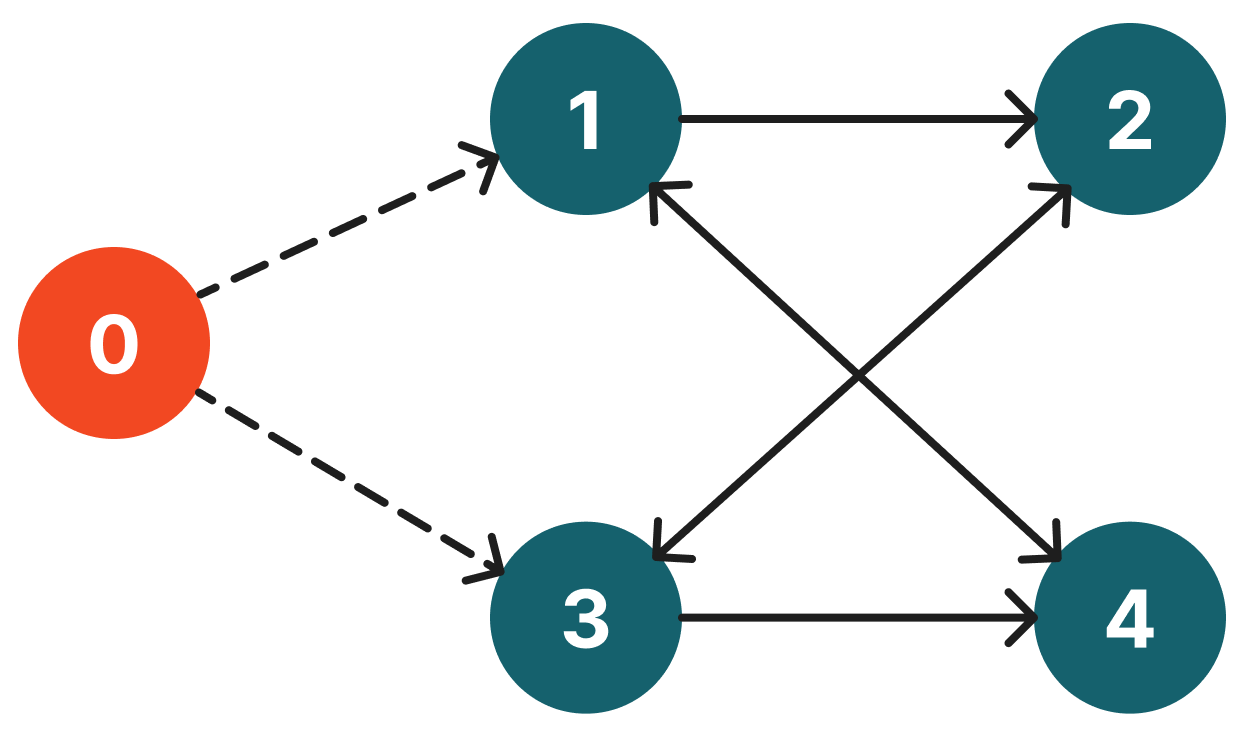
\includegraphics[width=0.6\textwidth]{communication.png}
    \caption{Communication topology among agents.}
    \label{fig:communication1} % Label for referencing the figure
\end{figure}

This section describes the methodology and hardware used for speed regulation, including the calculation of motor speed using the quadriple-frequency data processing  method.

\subsection{Hardware Implementation}

The DC brushed motors have a rated voltage of 12V, an unloaded speed of 293 ± 21 RPM, and a rated current of 0.36 A. The gear ratio of 20 means that the output speed of the motor is 1/20 of the rotor speed, resulting in higher torque with a higher gear ratio. The Hall encoders used have 13 pulses per revolution , meaning each full rotation generates 13 pulse signals. 

To enhance measurement accuracy, employing the quadruple-frequency data processing method. This technique quadruples the effective resolution of the encoder by processing the output pulse signals at four times the frequency, thus increasing measurement precision by a factor of four.

\subsection{Data Processing Method}

The motor speed is measured in revolution per sencond $(r/s)$ based on encoder measurements and the sampling interval $t$. The total number of encoder counts per revolution is calculated as $ T=4N_{e}R{r} $, where $N_e$ is the encoder line count equal to 13, $R_r$ is the reduction ratio equal to 20 and the factor of 4 accounts for quadrature encoding. The number of rotations, $N_r$ is determined using $N_r = \frac{m}{T}$, with $m$ representing the total encoder count.

The speed of the motor is then derived as:

\begin{equation}
           \label{motor_speed}
           v = \frac{N_r}{t} = \frac{m}{T  t}
\end{equation}



% The motor speed is measured in revolutions per second . The following equations are used to calculate the speed based on encoder measurements and sampling:

% 1. Calculation of Rounds:

%    The total number of rounds that the encoder measures is given by:
%    \begin{equation}
%        \label{model 32}
%        T = N_e \times R_r \times 4
%    \end{equation}
%    where $N_e$ is the encoder line count equal to 13, and $R_r$ is the reduction ratio equal to 20. The factor of 4 accounts for the quadrature encoding, which effectively quadruples the resolution.

% 2. Calculation of Number of Rotations:

%    The number of rotations can be determined using:
%    \begin{equation}
%        \label{model 33}
%        N_r = \frac{m}{ T}
%    \end{equation}
%    where \( m \) is the total count from the encoder, and T is the number of encoder counts per revolution, derived from (\ref{model 32}).

% 3. Calculation of Speed:

%    The speed of the motor in resolution per second (\( r/s \)) is given by:
%    \begin{equation}
%        \label{model 34}
%        v = \frac{N_r}{t}
%    \end{equation}
%    where, \( v \) represents the speed, and \( t \) is the time interval it takes to complete those rotations.

% 4. Combining the Equations:

%    Substituting (\ref{model 33}) into Equation (\ref{model 34}), we obtain:
%    \begin{equation}
%        \label{model 35}
%        v = \frac{m}{T \times t}
%    \end{equation}
%    The above final equation integrates encoder measurements and the sampling period to provide an accurate speed regulation.

Each sampling interval triggers an interrupt where the controller samples the motor speed and updates control commands accordingly.

The quadruple-frequency method,  is crucial for maximizing encoder measurement precision, resulting in more accurate speed control for the motor system.

Four follower DC motors and the models for each DC motor governed by:

\[
\begin{array}{c}
\text{DC Motor 1}: \quad y_1(k+1) = \frac{m u_1(k)}{0.1 T}\\
\text{DC Motor 2}: \quad y_2(k+1) = \frac{m u_2(k)}{0.1 T } \\
\text{DC Motor 3}: \quad y_3(k+1) = \frac{m u_3(k)}{0.3 T } \\
\text{DC Motor 4}: \quad y_4(k+1) = \frac{m u_4(k)}{0.3 T } 
\end{array}
\]


It is evident that the agents considered are heterogeneous, as the dynamics differ from one another. In this scenario, the dynamics are assumed to be unknown and are only provided here to generate the I/O data for the MASs. 

As illustrated in Fig. 2, the virtual leader is designated as vertex 0. It can be observed that only agents 1 and 3 can receive information from the leader, forming a strongly connected communication graph. Assume that the information exchange among agents is directed and fixed. The laplacian matrix of the graph is given as follows:

\[
    L = \begin{bmatrix}
    1 & 0 & 0 & -1 \\
    -1 & 2 & -1 & 0 \\
    0 & -1 & 1 & 0 \\
    -1 & 0 & -1 & 2
    \end{bmatrix}
\]

with \( D = \text{diag}(1, 0, 1, 0) \). We consider the following two different desired trajectories.




The expression for \( y_d(k) \) is:

\[
y_d(k) = 0.5 \sin\left(\frac{k \pi}{30}\right) + 0.3  \cos\left(\frac{k \pi}{10}\right)
\]

as \( k \) in the range \( 0 \leq k \leq 200 \).

The initial parameters are chosen as \(u_i(1)=0.1\), \(y_i(1)=0.1\) and \(\phi_i(0)=1 \) for all agents in this simulation ,\(\Gamma_{1}=\Gamma_{2}=0.15\) and \(\Gamma_{3}=\Gamma_{4}=0.45\), with \(T=0.1\), \(m=350\), \(\eta=1\), \(\mu=1\). The MFA Controller parameters are given as \(\rho=1\), \(\lambda=50\) and \(\alpha=1\) with \(\epsilon=10^{-5}\).
\begin{figure}[H]
    \centering
    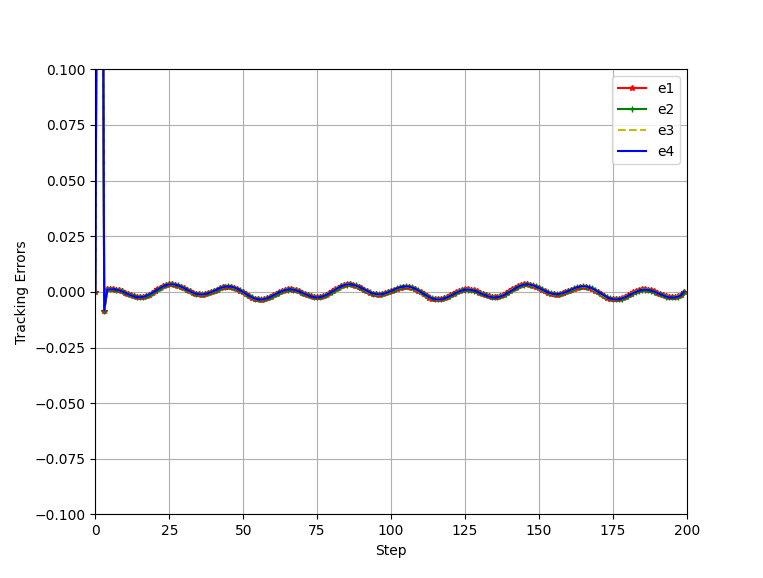
\includegraphics[width=0.6\textwidth]{Figure_2.png}
    \caption{Tracking errors for time varying desired trajectory.}
    \label{fig:figure_2} % Label for referencing the figure
\end{figure}

As shown in Fig. \ref{fig:figure_2}, the tracking errors between the actual and desired trajectories for agents $e_1$, $e_2$, $e_3$, and $e_4$ are relatively small and converge to zero over time. However, the individual agents exhibit varying levels of tracking error, suggesting that their unique dynamics or initial conditions may influence the performance.

\begin{figure}[H]
    \centering
    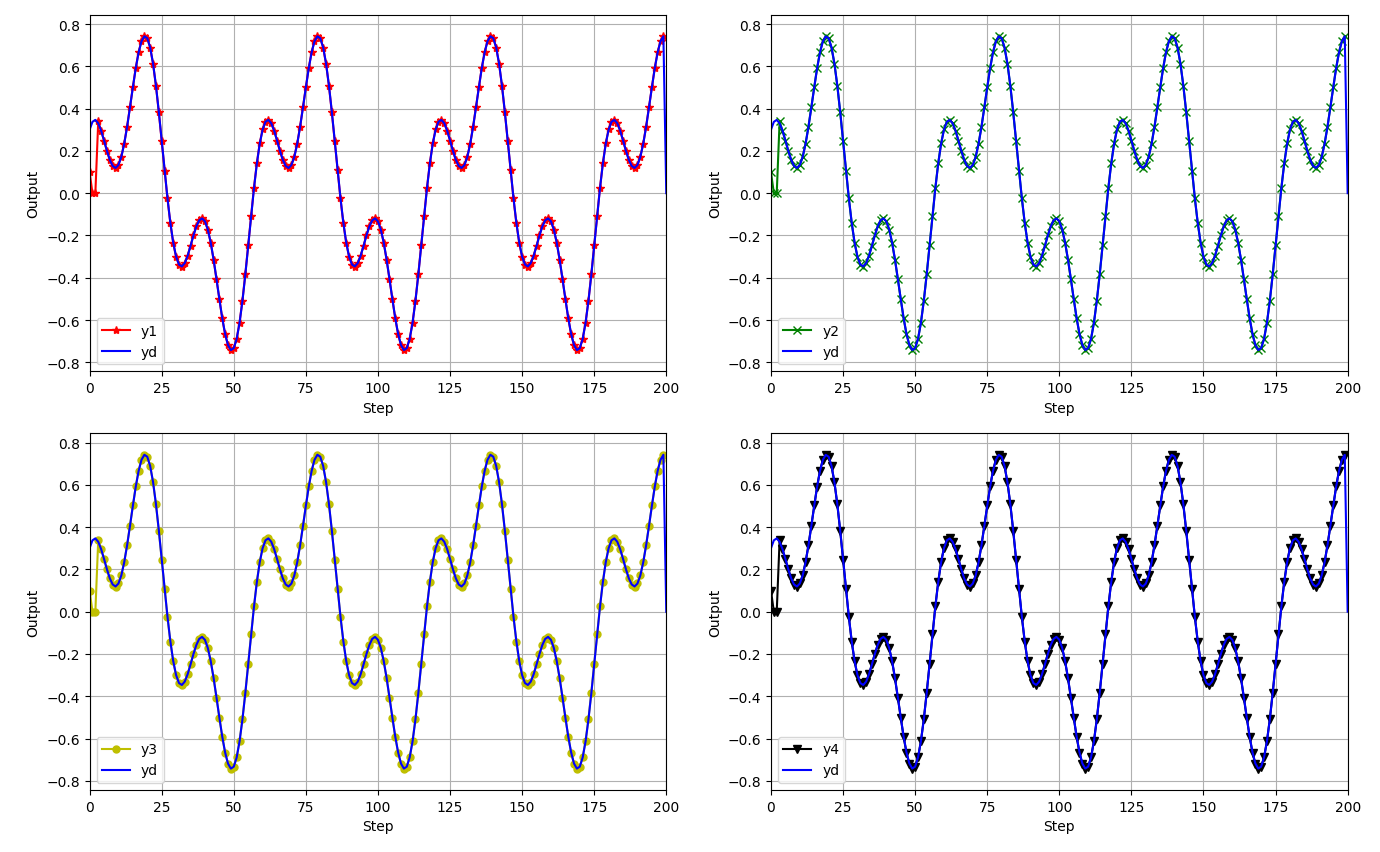
\includegraphics[width=0.9\textwidth]{Figure_1.png}
    \caption{Tracking performance of all agents for time-varying desired trajectory.}
    \label{fig:figure_3} % Label for referencing the figure
\end{figure}

Fig.\ref{fig:figure_3} presents a detailed analysis of the tracking performance for all agents. All agents successfully track the time-varying desired trajectory, confirming the effectiveness of the proposed control system. While minor variations in individual trajectories are evident, each agent generally adheres to the desired path. Factors such as agent dynamics, communication delays, and environmental disturbances could potentially influence the tracking performance.

\begin{figure}[H]
    \centering
    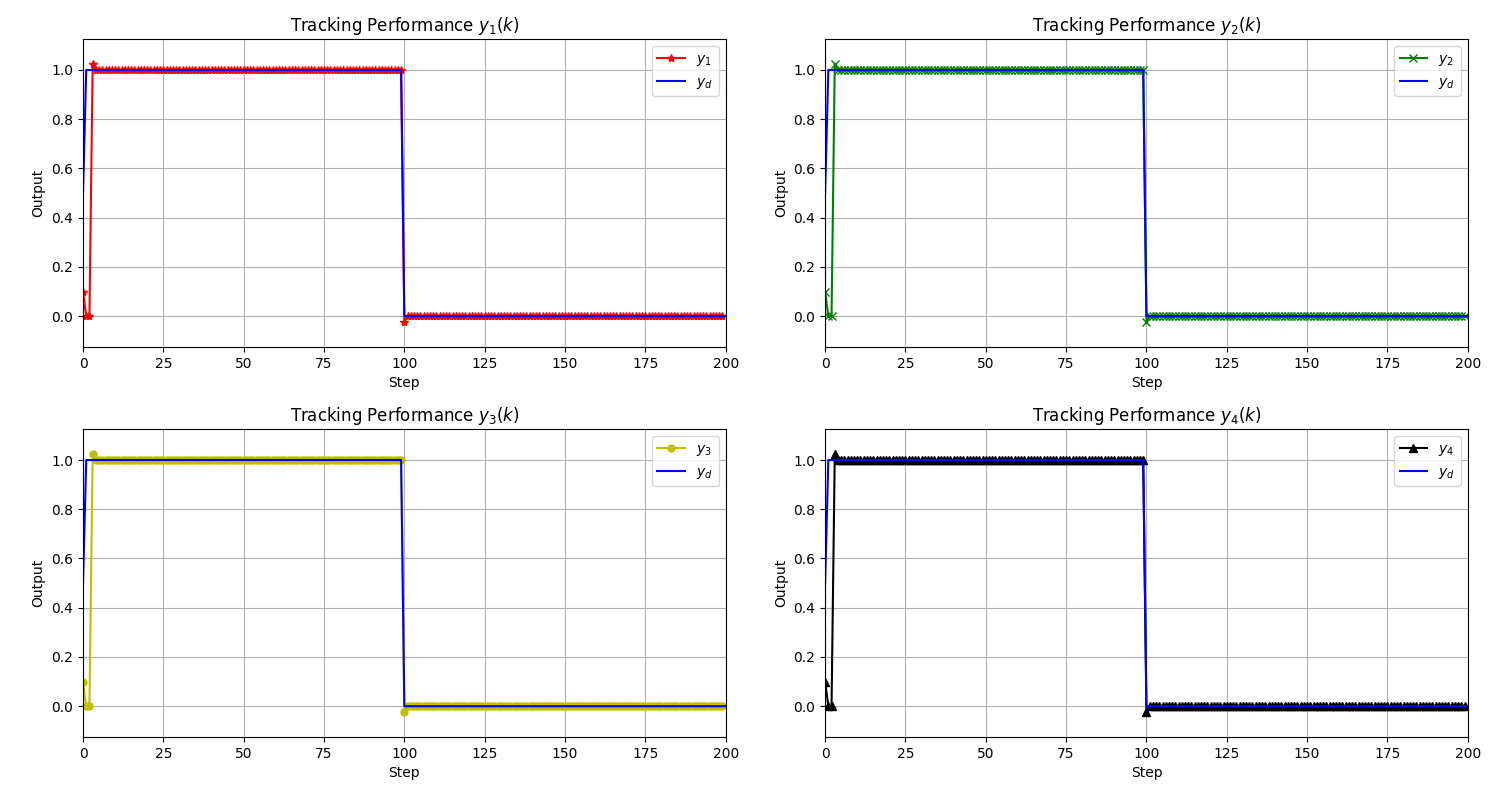
\includegraphics[width=0.8\textwidth]{Figure_4.png}
    \caption{Tracking performance of all agents for time-invariable desired trajectory.}
    \label{fig:figure_4} % Label for referencing the figure
\end{figure}

\begin{figure}[H]
    \centering
    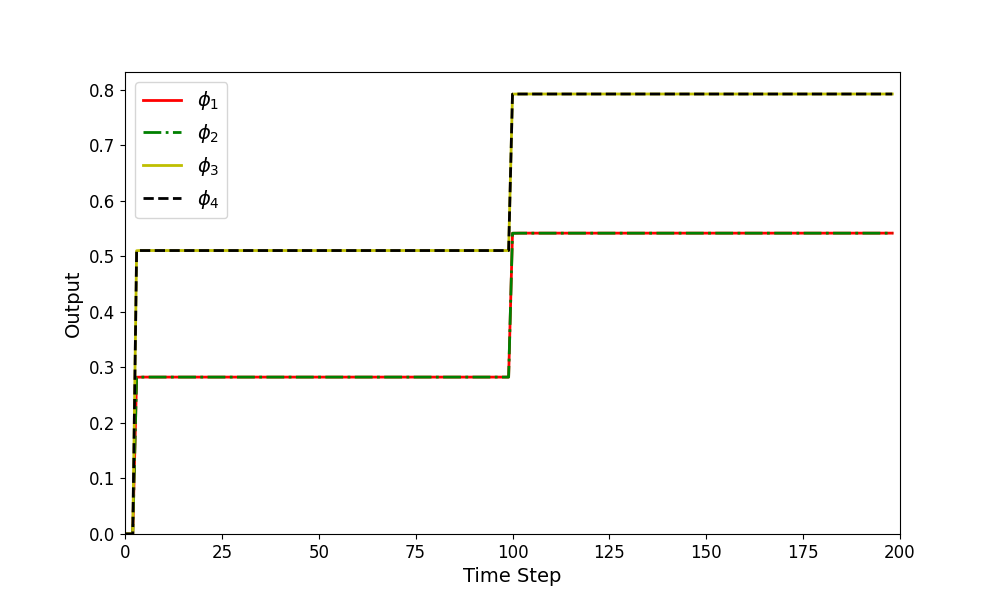
\includegraphics[width=0.7\textwidth]{Figure_5.png}
    \caption{PPD Estimation of all agents.}
    \label{fig:figure_5} % Label for referencing the figure
\end{figure}

Fig. \ref{fig:figure_4} demonstrates that all agents successfully track the time-invariable desired trajectory, further validating the robustness of the proposed control strategy. Meanwhile, Fig. \ref{fig:figure_5} shows the PPD estimation for all agents, highlighting the accuracy of the adaptive estimation process within the control framework.

\subsection{Physical verification}

The physical verification was conducted using a multi-DC motors system. The system consists of multi DC-motors system, an STM32F407ZET6 board, and is connected through two motor drivers. 

The reference trajectory is:

\[ y_d(k)=0.1(\pi)+0.25(\pi)\sin(0.25)+0.2 \]

The following figure shows the output results of the system.

\begin{figure}[H]
    \centering
    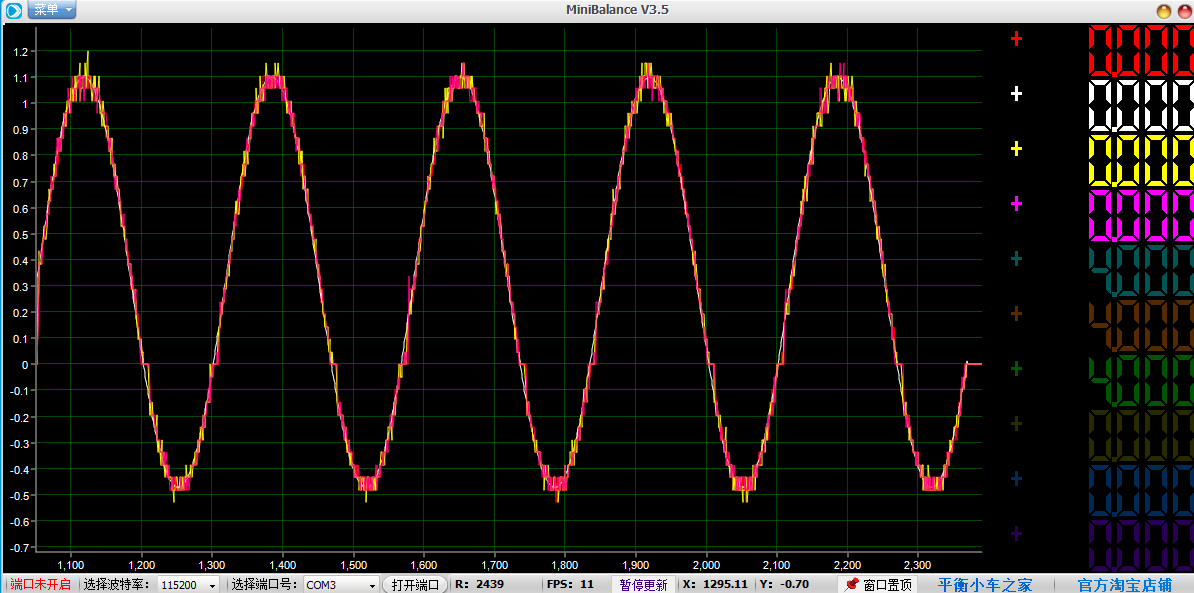
\includegraphics[width=0.8\textwidth]{output.png}
    \caption{Tracking performance of 3 DC motors for time-invariable desired trajectory.}
    \label{fig:output} % Label for referencing the figure
\end{figure}

Fig.\ref{fig:output} shows the tracking performance of multi-DC motors. As presented, all DC motors successfully track the desired trajectory, demonstrating the effectiveness of the proposed control method. Where the reference trajectory is presented by white color.

Overall, the simulation results suggest that the proposed control system is capable of tracking a constant desired trajectory for multiple agents. While there may be initial transient error, the system eventually reaches a steady-state condition with minimal tracking error. The variations in tracking performance among the agents highlight the potential influence of individual characteristics and external factors.

\section{Conclusion}

In this paper, a novel model-free adaptive sliding mode control was presented for multi-DC motors speed regulation. The proposed method achieves robust performance and adaptability in the presence of varying conditions. Utilizing a fixed topology represented by Laplacian matrice, the control strategy effectively manages the interconnections among multiple DC motors. The advantages and effectiveness of the proposed approach are demonstrated through detailed simulation results. Future work will focus on implementing the proposed approach in practical scenerios under hardware constraints.




% \begin{thebibliography}{99}
%     \bibitem{1}
%     Bu, XH; Hou, ZS and Zhang, HW. Data-Driven Multiagent Systems Consensus Tracking Using Model Free Adaptive Control.{\sl 
%     IEEE TRANSACTIONS ON NEURAL NETWORKS AND LEARNING SYSTEMS}, May 2018,29{\bf (5)}: 1514-1524.

%     \

%     \bibitem{2}

%     \

% \end{thebibliography}

\begin{thebibliography}{99}


    \bibitem{1}
    Lewis, F.L.; Zhang, H.; Hengster-Movric, K.; Das, A. Cooperative Control of Multi-Agent Systems: Optimal and Adaptive Control
    Design; Springer Science and Business Media: Berlin/Heidelberg, Germany, 2014.
    
    \bibitem{2}
    Bu, XH; Hou, ZS and Zhang, HW. Data-Driven Multiagent Systems Consensus Tracking Using Model Free Adaptive Control. \textit{IEEE Transactions on Neural Networks and Learning Systems}, May 2018, 29(5): 1514-1524.

    \bibitem{3}
    Ren, W. Consensus strategies for cooperative control of vehicle formations. IET Control Theory Appl. 2007, 1, 505–512.

    \bibitem{4}
    Dong, S.; Wang, C.; Wen, S.; Gang, F. A synchronization approach to trajectory tracking of multiple mobile robots while
    maintaining time-varying formations. IEEE Trans. Robot. 2009, 25, 1074–1086.
    
    \bibitem{5}
    Z. Hou and S. Jin, "A novel data-driven control approach for a class of SISO nonlinear systems," \textit{IEEE Transactions on Control Systems Technology}, vol. 19, no. 6, pp. 1549-1558, 2011.
    
    \bibitem{6}
    R. Olfati-Saber, J. A. Fax, and R. M. Murray, "Consensus and cooperation in networked multi-agent systems," \textit{Proceedings of the IEEE}, vol. 95, no. 1, pp. 215-233, 2007.
    
    \bibitem{7}
    M. Sampei, T. Tamura, T. Kobayashi, and N. Shibui, “Arbitrary path
    tracking control of articulated vehicles using nonlinear control theory,”
    IEEE Trans. Control Syst. Technol., vol. 3, no. 1, pp. 125–131, Mar. 1995.
    
    \bibitem{8}
    W. Ren, R. W. Beard, and E. M. Atkins, "Information consensus in multivehicle cooperative control," \textit{IEEE Control Systems}, vol. 27, no. 2, pp. 71-82, 2007.
    
    \bibitem{9}
    D. Xu, B. Jiang, and P. Shi, "Adaptive observer based data-driven control for nonlinear discrete-time processes," \textit{IEEE Transactions on Automation Science and Engineering}, vol. 11, no. 4, pp. 1037-1045, 2014.
    
    \bibitem{10}
    R. Chi, Z. Hou, S. Jin, D. Wang, and C.-J. Chien, "Enhanced data-driven optimal terminal ILC using current iteration control knowledge," \textit{IEEE Transactions on Neural Networks and Learning Systems}, vol. 26, no. 11, pp. 2939-2948, 2015.
    
    \bibitem{11}
    Ren, Y.; Hou, Z. Robust model-free adaptive iterative learning formation for unknown heterogeneous non-linear multi-agent systems. IET Control Theory Appl. 2020, 14, 654–663.
    
    \bibitem{12}
    C. L. P. Chen, G.-X. Wen, Y.-J. Liu, and F.-Y. Wang, "Adaptive consensus control for a class of nonlinear multiagent time-delay systems using neural networks," \textit{IEEE Transactions on Neural Networks and Learning Systems}, vol. 25, no. 6, pp. 1217-1226, 2014.
    
    \bibitem{13}
    Zhou, N (Zhou, Ning); Deng, WX (Deng, Wenxiang); Yang, XW (Yang, Xiaowei); Yao, JY (Yao, Jianyong), "Continuous adaptive integral recursive terminal sliding mode control for DC motors," \textit{International Journal of Control}, vol. 96, no. 9, pp. 2190-2200, June 2022.
    
    \bibitem{14}
    X. Liu, J. Lam, W. Yu, and G. Chen, "Finite-time consensus of multiagent systems with a switching protocol," \emph{IEEE Transactions on Neural Networks and Learning Systems}, vol. 27, no. 4, pp. 853–862, Apr. 2016.

    \bibitem{15}
    Z. Hou and Z. Wang, “From model-based control to data-driven control:
    Survey, classification and perspective,” Inf. Sci., vol. 235, pp. 3–35, 2013.

    \bibitem{16}
    Z. Hou and S. Jin, “A novel data-driven control approach for a class
    of discrete-time nonlinear systems,” IEEE Trans. Control Syst. Technol.,
    vol. 19, no. 6, pp. 1549–1558, Nov. 2011.

    \bibitem{17}
    D. Xu, B. Jiang, and F. Liu, “An improved data driven MDEL free adaptive
    constrained control for a solid oxide fuel cell,” IET Control Theory Appl.,
    vol. 10, no. 12, pp. 1412–1419, 2016.

    \bibitem{18}
    D. Xu, B. Jiang, and P. Shi, “A novel model free adaptive control design
    for multivariable industrial processes,” IEEE Trans. Ind. Electron., vol. 61,
    no. 11, pp. 6391–6398, Nov. 2014.

    \bibitem{19}
    D. Xu, B. Jiang, and P. Shi, “Adaptive observer based data-driven control
    for nonlinear discrete-time processes,” IEEE Trans. Autom. Sci. Eng.,
    vol. 11, no. 4, pp. 1037–1045, Oct. 2014.

    \bibitem{20}
    Z. Pang, G. Liu, D. Zhou, and D. Sun, “Data-based predictive control for networked nonlinear systems with network-induced delay and packet dropout,”IEEE Trans. Ind. Electron., vol. 63, no. 2, pp. 1249–1257,
    Feb. 2016.

    \bibitem{21}
    H. Zhang and F. L. Lewis, ”Adaptive cooperative tracking control of higher-order nonlinear systems with unknown dynamics,” Automatica, vol. 48, no.
    7, pp. 1432-1439, 2012.

    \bibitem{22}
    J. Liu, S. Vazquez, L. Wu, A. Marque, H. Gao, and L. G. Franquelo
    et al., “Extended state observer based sliding mode control for three-phase
    power converters,” IEEE Trans. Ind. Electron., vol. 64, no. 1, pp. 22–31,
    Jan. 2017.
    
    \bibitem{23}
    Z.-G. Hou, L. Cheng, and M. Tan, "Decentralized robust adaptive control for the multiagent system consensus problem using neural networks," \emph{IEEE Transactions on Systems, Man, and Cybernetics, Part B: Cybernetics}, vol. 39, no. 3, pp. 636–647, Jun. 2009.
    
    \bibitem{24}
    Z. Hou and W. Huang, "The model-free learning adaptive control of a class of SISO nonlinear systems," \emph{Proceedings of the American Control Conference}, Albuquerque, NM, USA, Jun. 1997, pp. 343–344.
    
    \bibitem{25}
    H. Su, G. Chen, X. Wang, and Z. Lin, "Adaptive second-order consensus of networked mobile agents with nonlinear dynamics," \emph{Automatica}, vol. 47, no. 2, pp. 368–375, Feb. 2011.
    
    \bibitem{26}
    D. Xu, B. Jiang, and P. Shi, "Adaptive observer based data-driven control for nonlinear discrete-time processes," \emph{IEEE Transactions on Automation Science and Engineering}, vol. 11, no. 4, pp. 1037–1045, Oct. 2014.
    
    \bibitem{27}
    H. Zhang and F. L. Lewis, "Adaptive cooperative tracking control of higher-order nonlinear systems with unknown dynamics," \emph{Automatica}, vol. 48, no. 7, pp. 1432–1439, Jul. 2012.
    
    \bibitem{28}
    Z. Wu, X. Wang, and X. Zhao, “Backstepping terminal sliding mode
    control of DFIG for maximal wind energy captured,” Int. J. Innovative
    Comput. Inf. Control, vol. 12, no. 5, pp. 1565–1579, 2016.

    \bibitem{29}
    X. Yan and C. Edwards, “Adaptive sliding-mode-observer-based fault
    reconstruction for nonlinear systems with parametric uncertainties,” IEEE
    Trans. Ind. Electron., vol. 55, no. 11, pp. 4029–4036, Nov. 2008.

    \bibitem{30}
    J. Liu, W. Luo, X. Yang, and L. Wu, “Robust model-based fault diagnosis
    for PEM fuel cell air-feed system,” IEEE Trans. Ind. Electron., vol. 63,
    no. 5, pp. 3261–3270, May 2016.

    \bibitem{31}
    A. Anuchin, A. Dianov and F. Briz, "Synchronous Constant Elapsed Time Speed Estimation Using Incremental Encoders," in IEEE/ASME Transactions on Mechatronics, vol. 24, no. 4, pp. 1893-1901, Aug. 2019, doi: 10.1109/TMECH.2019.2928950.

    \bibitem{32}
    S. Qin and T. Badgwell, “A survey of industrial model predictive control
    technology,” Control Eng. Pract., vol. 11, pp. 733–764, 2003.

    \bibitem{32}
    A. Sharafian, V. Bagheri, and W. Zhang, "RBF neural network sliding mode consensus of multi-agent systems with unknown dynamical model of leader-follower agents," \textit{International Journal of Control, Automation and Systems}, vol. 16, no. 2, pp. 749–758, 2018.

    \bibitem{33}
    X. Ma, F. Sun, H. Li, and B. He, "Neural-network-based integral sliding-mode tracking control of second-order multi-agent systems with unmatched disturbances and completely unknown dynamics," \textit{International Journal of Control, Automation and Systems}, vol. 15, no. 4, pp. 1925–1935, 2017.
    

    \bibitem{34}
    R. Rahmani, H. Toshani, and S. Mobayen, "Consensus tracking of multi-agent systems using constrained neural-optimiser-based sliding mode control," \textit{International Journal of Systems Science}, vol. 51, no. 14, pp. 2653–2674, 2020.

    \bibitem{35}
    Z. Peng, G. Wen, A. Rahmani, and Y. Yongguang, "Distributed consensus-based formation control for multiple nonholonomic mobile robots with a specified reference trajectory," \textit{International Journal of Systems Science}, vol. 46, no. 8, pp. 1447–1457, 2015.
    
    \end{thebibliography}
    


\end{document}